\begin{figure}[t]
\centering
% Vector drawing generated by tools/figures/relbench_cumulative.py from exp/2026-10-20-relbench/paper-sessions.json; rerun it after the numbers change.
\ifbilingual
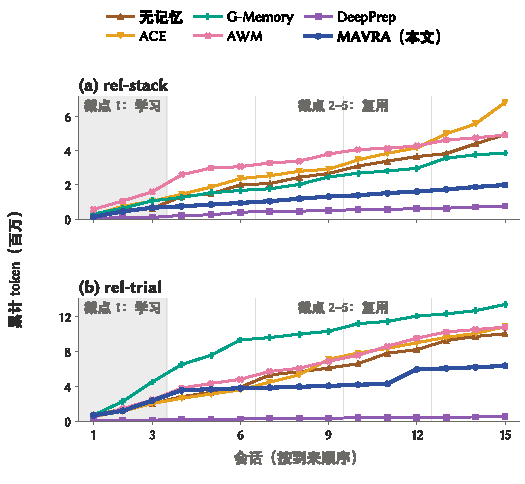
\includegraphics[width=\linewidth]{figures/relbench-cumulative-zh}
\else
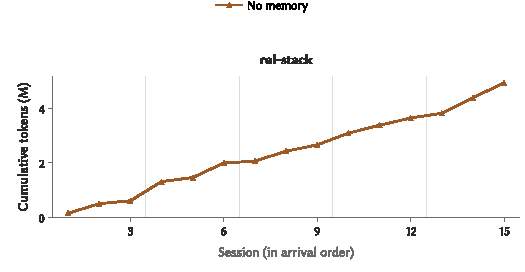
\includegraphics[width=\linewidth]{figures/relbench-cumulative}
\fi
\caption{\bt{Cumulative tokens of the RelBench sessions in arrival order, memory operations included; thin rules separate the five cutoffs. After the first cutoff, \system's agents start from the verified task program and its curve flattens, while the other methods keep paying for exploration at every cutoff.}{按到来顺序累计的 RelBench 会话 token（含记忆操作）；细线分隔 5 个截点。第一个截点之后，\system\ 的智能体从经验证的任务方案出发，曲线变平；其他方法在每个截点都继续为探索付费。}}
\label{fig:relbench-cumulative}
\Description{Two line charts, rel-stack and rel-trial, of cumulative tokens in millions against the session index from 1 to 15, one line per method.}
\end{figure}
